\documentclass[a4paper,11pt,oneside]{book}

% slovenske pisanie
\usepackage[utf8]{inputenc}
\usepackage[T1]{fontenc}
\usepackage[slovak]{babel}

% mensie okraje
\usepackage{geometry}
\geometry{margin=1in}

\usepackage{amssymb}
\usepackage{amsmath}

\usepackage{amsthm}
\theoremstyle{plain}
\newtheorem{theorem}{Veta}[chapter]
\newtheorem{lemma}[theorem]{Lemma}
\newtheorem{proposition}[theorem]{Tvrdenie}
\newtheorem{corollary}[theorem]{Dôsledok}
\theoremstyle{remark}
\newtheorem{remark}{Poznámka}[chapter]
\theoremstyle{definition}
\newtheorem{definition}{Definícia}
\newtheorem{assumption}{Predpoklad}
\newtheorem{exercise}{}[chapter]

\usepackage{xcolor} % \color
\usepackage{graphicx} % obrazky
\usepackage{subcaption} % \subfigure
\usepackage{hyperref} % linky
\usepackage{comment} % \comment

\newcommand{\err}{\mathrm{err}}
\newcommand{\Err}{\mathrm{Err}}
\newcommand{\norm}[1]{\left\lVert#1\right\rVert}

\newcommand{\N}{\mathbb{N}}
\newcommand{\R}{\mathbb{R}}
\newcommand{\C}{\mathbb{C}}

\DeclareMathOperator*{\argmin}{{arg\,min}}
\DeclareMathOperator*{\prob}{\mathrm{Pr}}
\DeclareMathOperator*{\E}{\mathrm{E}}
\DeclareMathOperator*{\Var}{\mathrm{Var}}
\DeclareMathOperator*{\Cov}{\mathrm{Cov}}

\newcommand{\vychylka}{{\epsilon_\text{approx.}}}
% \newcommand{\vychylkaT}{{\epsilon^T_\text{approx.}}}
\newcommand{\rozptyl}{{\epsilon_\text{est.}}}
\newcommand{\rozptylT}{{\epsilon^T_\text{est.}}}

\newcommand{\larr}{\leftarrow}
\newcommand{\rarr}{\rightarrow}
\newcommand{\uarr}{\uparrow}
\newcommand{\darr}{\downarrow}


\newcommand{\TODO}[1]{\noindent {\color{red} TODO #1} \\}


\begin{document}
  
  \tableofcontents
  \newpage
  
  \chapter{Teória strojového učenia I}

Chceme sa naučiť na základe nejakých vstupných dát $x$ predikovať $y$.
Môžeme si to predstaviť tak, že príroda vie poskytovať pozorovania,
každé v tvare dvojice $(x, y)$. Dostali sme od nej sadu $t$ pozorovaní,
na základe ktorých chceme navrhnúť nejakú funkciu $h$, ktorá predpovedá
$y$ na základe $x$. Dobrá funkcia je taká, ktorá je schopná
\emph{zovšeobecňovať}, teda sa jej ``dobré darí'' aj na dátach mimo
trénovacej množiny. Proces, ktorým $h$ zostrojíme, si môžeme predtaviť
ako algoritmus, ktorý berie ako vstupy trénovacie dáta a vráti nám
funkciu.




\section{Matematický model}

Z matematického hľadiska, prírodu vieme formalizovať ako
pravdepodobnostnú distribúciu $P$. Množinu všetkých možných
$x$ označíme $X$, množinu možných $y$ označíme $Y$.

V tejto časti sa nebudeme zaoberať výpočtovou stránkou strojového
učenia, od detailov ako časová zložitosť, ..., abstrahujeme. Algoritmus
si teda predstavíme iba ako niečo, čo vezme ako vstup trénovacie dáta
$(x_1, y_1), \ldots, (x_t, y_t)$ a na výstup vráti funkciu
$h : X \to Y$. Túto funkciu budeme volať \emph{hypotéza}. Množinu
všetkých možných funkcii, ktoré môže náš algoritmus vrátiť,
budeme volať \emph{množina hypotéz} a značiť ho $H$.

\paragraph{Chyba hypotézy.}
Ako vyjadriť mieru toho, že sa funkcii ``dobre darí''? Spravíme tak
pomocou \emph{chybovej funkcie} $\err : Y \times Y \to \reals^+$,
ktorej význam je nasledovný: $\err(y, y')$ vyjadruje, ako veľmi
sa od seba líšia $y$ a $y'$. Pomocou tejto funkcie vieme odmerať
priemernú chybu hypotézy $h$, ktorú budeme tiež označovať $\err$,
nasledovne:
$$\err(h) = \E_{x, y} \left[ \err(h(x), y) \right]$$
Pod $\E_{x, y}$ sa rozumie stredná hodnota cez $(x, y)$
z pravdepodobnostnej distribúcie $P$, teda $(x, y) \sim P$.
Pri klasifikácii sa zvykne používať chybová funkcia
$$
  \err(y, y') = \left\{
    \begin{array}{ll}
      0, & \text{ak}\ y = y' \\
      1, & \text{inak}
    \end{array}
  \right.
$$
a potom zrejme
$$\E_{x, y} \left[ \err(h(x), y) \right] = \prob_{x, y} \left( h(x) \neq y \right).$$
Pri regresii máme viacero možností, bežné voľby sú kvadratická chyba
$(y - y')^2$ a absolútna chyba $|y - y'|$.

\paragraph{Chyba algoritmu.}
Ako vyjadriť chybu celého učiaceho algoritmu? Uvedomme si, že výstup
algoritmu je závislý od trénovacích dát $T = \{(x_1, y_1), \ldots, (x_t, y_t)\}$,
ktoré dostane. Takže výstupná funkcia je od nich závislá, budeme ju
označovať $\hat{h}$. Potom priemerná chyba algoritmu (alebo inak
\emph{priemerná chyba priemernej hypotézy}), braná cez všetky možné
vzorky trénovacích dát, je rovná
$$\E_T \left[ \err(\hat{h}) \right] = \E_T \left[ \E_{x,y} \left[ \err(\hat{h}(x), y) \right] \right].$$
Pod $\E_T$ sa rozumie stredná hodnota cez všetky možné $t$-tice
trénovacích dát $T$, brané nezávisle z pravdepodobnostnej
distribúcie $P$.

\paragraph{Trénovacia chyba.}
Pri vyššie uvedených chybách sme vždy merali vzhľadom na skutočnú
distribúciu $P$. Môže nás ale zaujímať, aká je priemerná chyba
hypotézy na trénovacích dátach $T$. Túto chybu budeme označovať
$\err_T(h)$, a vypočítame ju ako
$$\err_T(h) = \E_{x_i, y_i} \left[ \err(h(x_i), y_i) \right] = \frac{1}{t} \cdot \sum_{i=1}^t \err(h(x_i), y_i).$$

Priemerná trénovacia chyba z pohľadu algoritmu bude
$$\E_T \left[ \err_T(\hat{h}) \right].$$

V nasledujúcom texte budeme vynechávať premenné, cez ktoré prebiehajú
stredné hodnoty, všade tam, kde budú zrejmé z kontextu.




\section{Analýza veľkostí chýb}

V tejto časti sa podrobnejšie pozrieme na to, ako závisia vyššie
uvedené štatistiky (tj. priemerná testovacia a trénovacia chyba
priemernej hypotézy) od veľkosti trénovacej množiny $T$ a od veľkosti
množiny hypotéz $H$.

V celej časti budeme predpokladať, že úloha je regresného
charakteru a chyba sa meria ako kvadratická odchýlka, teda
$$\err(y, y') = (y - y')^2.$$



\subsection{Teoretické limity}
Najprv sa ale pozrieme na teoretické limity toho, ako dobrá vôbec
môže nejaká funkcia byť. Označme $h^{\square}$ najlepšiu možnú funkciu,
nemusí byť nutne z $H$. Teda
$$h^{\square} = \argmin_h \left( \err(h) \right) = \argmin_h \left( \E_{x,y} \left[ (h(x) - y)^2 \right] \right).$$
Jediné obmedzenia kladené na $h$ sú, že je to funkcia: pre každé $x$
musí vrátiť vždy jednu a tú istú hodnotu. Distribúcia $P$ ale nemusí
pre dané $x$ vždy vrátiť to isté $y$: môže byť zašumená, alebo
jednoducho $x$ neobsahuje dostatočnú informáciu. Napríklad, ak podľa
plochy bytu určujeme jeho cenu, niektoré dva byty môžu mať rovnakú
plochu a predsa rôznu cenu. Ako uvidíme, tento nedeterminizmus je
jediný dôvod, prečo hypotéza $h^{\square}$ nemusí mať nulovú chybu.

Chybu ľubovoľnej hypotézy $h$ vieme upraviť nasledovne:
\begin{align}
  \err(h)
    &= \E_{x,y} \left[ (h(x) - y)^2 \right] \\
    &= \E_{x} \left[ \E_{y|x} \left[ (h(x) - y)^2 \right] \right]
\end{align}
Pozrime sa na vnútornú strednú hodnotu. V nej je $x$ konštanta, a
teda aj $h(x) = c$ je konštanta. Aká konštanta minimalizuje danú
strednú hodnotu? Nie je ťažké vidieť (napríklad zderivovaním), že
minimum sa nadobúda pre $c = \E[y]$. Takže
$$h^{\square}(x) = \E_{y|x}[y],$$
a jeho priemerná chyba je
$$\err(h^{\square}) = \E_{x} \left[ \E_{y|x} \left[ (y - \E[y]) \right] \right] = \E_{x} \left[ \Var_{y|x}(y) \right].$$
Vidíme teda, že pokiaľ je $y$ jednoznačne určené $x$-om, tak
$h^{\square}$ bude mať nulovú chybu.



\subsection{Bias-variance tradeoff}
V tomto odseku si ukážeme zaujímavý výsledok, ktorý nám za určitých
predpokladov umožňuje vyjadriť chyby pomocou iných, jasnejších veličín:
tzv. \emph{výchylky} a \emph{rozptylu}.


\paragraph{Odvodenie.}
Označme najlepšiu hypotézu z množiny $H$ ako $h^\star$, teda
$$h^\star = \argmin_h \left( \err(h) \right).$$

Budeme upravovať výraz reprezentujúci priemernú chybu priemernej
hypotézy $\hat{h}$.
\begin{align}
  \chalg % \E_T \left[ \err(\hat{h}) \right]
    &= \E_T \left[ \err(\hat{h}) \right] \\
    &= \E_T \left[ \E_{x,y} \left[ (\hat{h}(x) - y)^2 \right] \right] \\
    &= \E_T \left[ \E_{x,y} \left[ \left( (\hat{h}(x) - h^\star(x)) + (h^\star(x) - y) \right)^2 \right] \right]
\end{align}
V tomto momente prichádza netriviálny technický krok, ktorý si
vyžaduje dodatočné predpoklady. Tieto technické detaily prenecháme
na koniec časti, sústreďme sa na to hlavné.
$$
  \chalg
    = \E_T \left[ \E_{x,y} \left[ (\hat{h}(x) - h^\star(x))^2 \right] \right]
    + \E_T \left[ \E_{x,y} \left[ (h^\star(x) - y)^2 \right] \right]
$$
Druhý zo sčítancov sa dá ešte zjednodušiť. Kedže $h^\star$ ani $y$
nezávisia od trénovacích dát, môžeme sa zbaviť vonkajšej strednej
hodnoty. Dostávame tak výslednú rovnosť
$$
  \chalg
    = \underbrace{\E_T \left[ \E_{x,y} \left[ (\hat{h}(x) - h^\star(x))^2 \right] \right]}_{\text{rozptyl}}
    + \underbrace{\E_{x,y} \left[ (h^\star(x) - y)^2 \right]}_{\text{výchylka}}.
$$

Prvý zo sčítancov budeme volať \emph{rozptyl}. Trénovací algoritmus
s malým rozptylom vracia funkcie, ktoré sú blízko optima v množine $H$.
Tým, že mu zväčšíme množinu trénovacích dát, si veľmi neprilepšíme.
Naopak, algoritmus s veľkým rozptylom vracia funkcie ďaleko od optima,
teoreticky by sme sa teda vedeli k optimu priblížiť tým, že zväčšíme
množstvo trénovacích dát.

\medskip

Druhý zo sčítancov budeme volať \emph{výchylka}. Vyjadruje chybu, ktorá
je spôsobená tým, že sa náš algoritmus obmedzil na nejakú konkrétnu
množinu hypotéz $H$. Čím väčšia množina hypotéz, tým menšia výchylka
(nakoľko $h^\star$ je najlepšia hypotéza v množine $H$, jej zväčšením
si môžeme iba prilepšiť). Zložitejšia množina hypotéz ale ľahšie
``napasuje'' na ľubovoľné trénovacie dáta. To zvyšuje riziko toho,
že výsledná hypotéza bude špecifická pre obdržané dáta, a nebude
schopná zovšeobecňovať mimo nich. Je teda potreba väčšieho množstva
trénovacích dát.

\medskip

Ak máme fixné trénovacie dáta $T$, pri voľbe množiny hypotéz $H$ sa snažíme
nájsť kompromis medzi malým rozptylom a malou výchylkou. Zložité $H$
bude mať malú výchylku ale veľký rozptyl, čo vedie k tzv. \emph{preučeniu}.
Jednoduché $H$ bude mať malý rozptyl, ale veľkú výchylku, tzv. \emph{podučenie}.

Na obrázku \ref{img:fitting} ilustrujeme oba koncepty: úlohou je modelovať
kvadratickú funkciu. Ak za množinu hypotéz zvolíme lineárne funkcie,
ich chyby sa nebudú veľmi od seba líšiť, ale všetky budú zle. Ak za
množinu hypotéz zvolíme polynómy nejakého vysokého stupňa, ľahko
nájdeme polynóm prechádzajúci cez trénovacie dáta, avšak mimo nich
bude dávať výsledky úplne mimo.

\begin{figure}
  \centering
  \begin{subfigure}[b]{0.3\linewidth}
    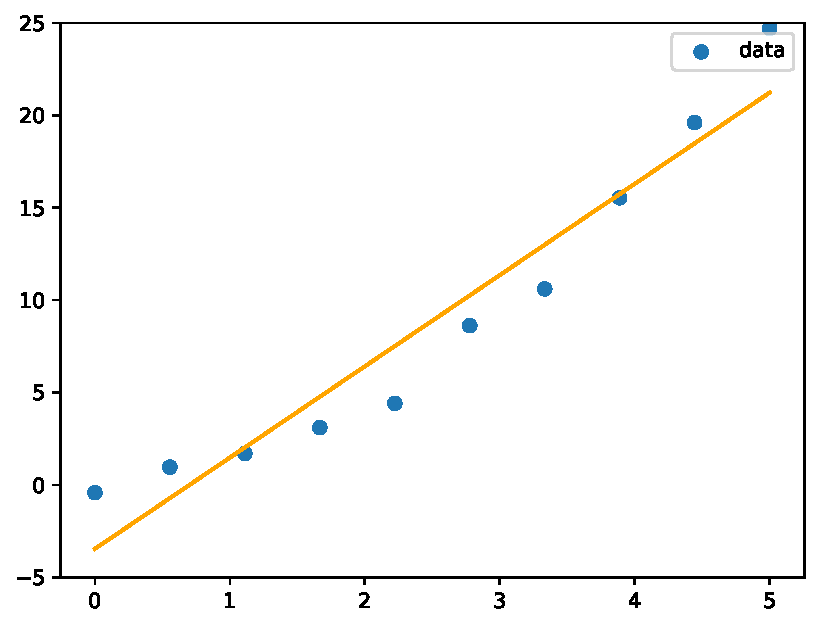
\includegraphics[width=\linewidth]{obrazky/fitting1.pdf}
  \end{subfigure}
  ~
  \begin{subfigure}[b]{0.3\textwidth}
    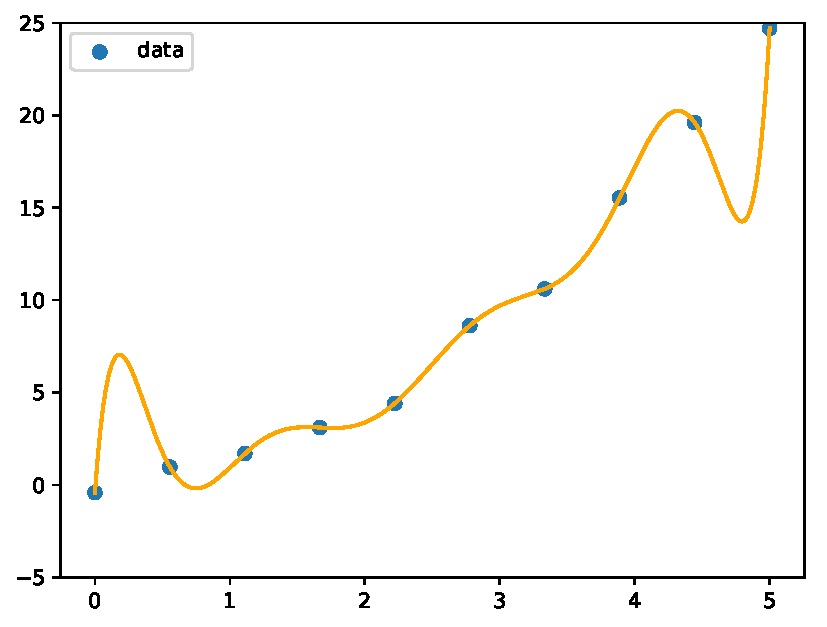
\includegraphics[width=\linewidth]{obrazky/fitting9.pdf}
  \end{subfigure}
  ~
  \begin{subfigure}[b]{0.3\textwidth}
    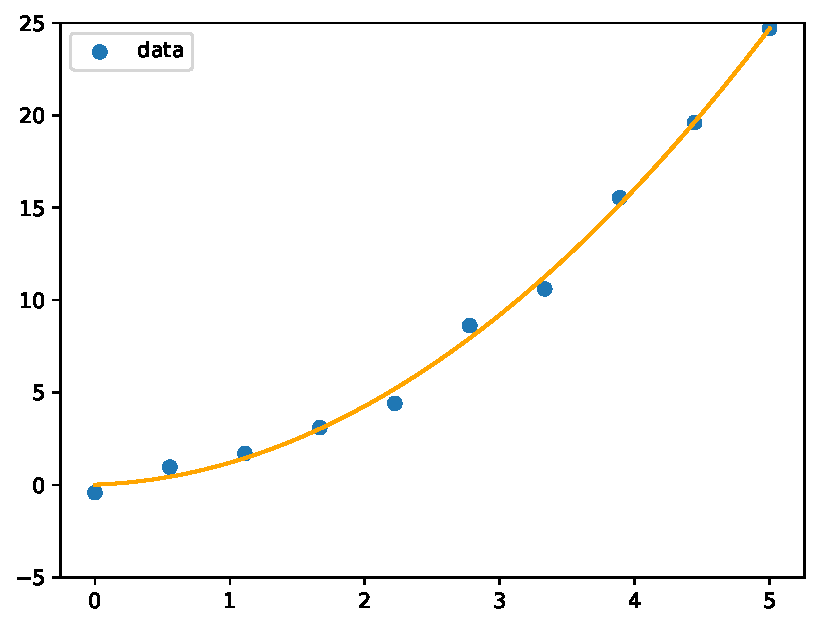
\includegraphics[width=\linewidth]{obrazky/fitting2.pdf}
  \end{subfigure}
  \caption{Podučenie, preučenie, akurát.}
  \label{img:fitting}
\end{figure}

\medskip

Výchylku vieme upraviť ďalej. Hypotéza $h^\star$ ani $y$ nezávisia
od trénovacej množiny $T$. Z ich pohľadu sú teda testovacie dáta $x, y$
a trénovacie dáta $x_i, y_i$ nerozoznateľné. Takže na meranie chyby
$h^\star$ môžeme použiť trénovacie dáta (berúc v úvahu ich náhodný
výber):
\begin{align}
  \vychylka
    &= \E_T \left[ \E_{x_i, y_i} \left[ (h^\star(x_i) - y_i)^2 \right] \right] \\
    &= \E_T \left[ \E_{x_i, y_i} \left[ \left( (h^\star(x_i) - \hat{h}(x_i)) + (\hat{h}(x_i) - y_i) \right)^2 \right] \right]
\end{align}
Použitím ďalšieho technického kroku dostaneme:
\begin{align}
  \vychylka &= \underbrace{\E_T \left[ \E_{x_i, y_i} \left[ (h^\star(x_i) - \hat{h}(x_i))^2 \right] \right]}_{\text{trénovací rozptyl}}
    + \underbrace{\E_T \left[ \E_{x_i, y_i} \left[ (\hat{h}(x_i) - y_i)^2 \right] \right]}_{\text{priemerná trénovacia chyba}}
\end{align}

Prvý zo sčítancov budeme volať \emph{trénovací rozptyl}.
Uvedomme si, že pre ľubovoľné trénovacie dáta $T$ platí
$$\err_T(\hat{h}) \leq \err_T(h^\star),$$
nakoľko $\hat{h}$ je optimálna hypotéza pre danú množinu trénovacích
dát. Hypotéza $h$ síce je najlepšia pre $H$, trénovacie dáta sú ale len
malá vzorka z $H$.
Trénovací rozptyl teda môžeme chápať ako mieru toho, ako veľmi
reprezentatívnu vzorku trénovacích dát sme dostali. Čím menší je,
tým viac reprezentatívna vzorka je.

\medskip

Druhý zo sčítancov budeme volať \emph{priemerná trénovacia chyba}.
Je to priemerná chyba, ktorej sa dopustí výstu z algoritmu $\hat{h}$
na tých istých dátach, pomocou ktorých sme $\hat{h}$ zostrojili.

\medskip

Platí
$$ {\normalfont \text{priemerná trénovacia chyba}} \leq \vychylka \leq \chalg. $$
Na konkrétnych trénovacích dátach ale nemusí platiť, že trénovacia
chyba je menšia ako testovacia chyba: mohli sme si (síce s malou
pravdepodobnosťou, ale predsa) vytiahnuť zlé trénovacie dáta, ktoré
sa výrazne líšia od skutočných dát.

\medskip

Na základe dosiaľ uvedeného vieme graficky znázorniť, ako sa zhruba správajú
rozptyl, výchylka, trénovací rozptyl a priemerná trénovacia chyba,
v závislosti od veľkosti trénovacej množiny (obrázok \ref{img:train})
a od zložitosti množiny hypotéz (obrázok \ref{img:hypo}).


\TODO{obrázok kriviek učenia, vysvetlenie}


\paragraph{Technické detaily.}
Nakoniec sa vyjadríme k spomínanému technickému kroku. Začneme jeho
znením a potom uvedieme jeho predpoklady.

\begin{theorem} \label{theorem:proj1}
  Predpokladajme, že vstupom do hypotéz sú vektory reálnych čísel
  (tj. $X = \reals^n$), cieľom je predpovedať jedno reálne číslo
  (tj. $Y = \reals$), a že pravdepodobnostné rozdelenie $P$ je spojité.
  
  Nech množina hypotéz $H$ je uzavretá na lineárne kombinácie a na
  limity (teda ak postupnosť funkcii v $H$ konverguje, jej limita
  je tiež v $H$).
  
  Ďalej predpokladajme, že trénovací algoritmus vždy vráti takú funkciu
  $\hat{h} \in H$, ktorá minimalizuje trénovaciu chybu. Inak zapísané,
  $$\hat{h} = \argmin_{h \in H} \left( \E_T \left[ \err_T(h) \right] \right).$$
  
  Potom platí
  $$\E_T \left[ \E_{x,y} \left[ \left( (\hat{h}(x) - h^\star(x)) + (h^\star(x) - y) \right)^2 \right] \right] = \E_T \left[ \E_{x,y} \left[ (\hat{h}(x) - h^\star(x))^2 \right] \right] + \E_T \left[ \E_{x,y} \left[ (h^\star(x) - y)^2 \right] \right]$$
\end{theorem}
\begin{remark}
  Dokazovaná rovnosť je ekvivalentná s nasledovnou, stručnejšou:
  $$\E_T \left[ \E_{x, y} \left[ (\hat{h}(x) - h^\star(x)) \cdot (h^\star(x) - y) \right] \right] = 0.$$
  Túto kratšiu verziu získame roznásobením a použitím linearity strednej
  hodnoty. V dôkaze budeme dokazovať túto rovnosť.
\end{remark}
\begin{remark}
  Všimnite si, že potrebujeme uzavretosť množiny $H$ na limity na to,
  aby vôbec $\argmin_{h \in H} (\ldots)$ existovalo. Vo všeobecnosti
  nemusí existovať taká funkcia, ale môže existovať nekonečná postupnosť
  funkcii, každá ďalšia lepšia, ako tá predchádzajúca. (Inak povedané,
  neexistuje minimum, iba infimum.)
\end{remark}
\begin{remark}
  Je namieste otázka, či je $\argmin_{h \in H} (\ldots)$ dobre definované,
  teda či je taká funkcia $h$ práve jedna. Za chvíľu uvidíme, že naše
  predpoklady to zaručujú.
\end{remark}
\begin{remark}
  Veta by sa dala rozšíriť aj na iné množiny $X, Y$, napríklad keď
  predpovedaná premenná je vektor ($Y = \reals^m$), ... Možno ani $P$
  nemusí byť spojité. Pre jednoduchosť argumentu ale budeme uvažovať
  vetu tak, ako je popísaná vyššie.
\end{remark}
\begin{remark}
  Predpoklady vety sú značne obmedzujúce. Napríklad si uvedomte, že
  ju nie je možné použiť na klasifikáciu, či dokonca ani na ľubovoľnú
  ohraničenú regresiu (kde rozumné hodnoty $y$ sú ohraničené). Ale taká
  je teória.
\end{remark}

Pri našom dôkaze využijeme niekoľko vlastností funkcii, ktoré uvádzame
v nasledujúcom odseku. Skúsený čitateľ-matematik ho môže preskočiť.

\begin{definition}
  (Skalárny súčin.) Nech $f, g$ sú funkcie z $X$ do $\reals$,
  z nejakej príjemne sa správajúcej množiny funkcii (tj. rovnomerne
  spojité, ..., čokoľvek, aby nasledujúce argumenty prešli). Definujeme
  ich skalárny súčin $\langle \cdot, \cdot \rangle$ ako
  \begin{align}
    \langle f, g \rangle
      &= \int f(x) \cdot g(x)\ d\rho x \\
      &= \E_x \left[ f(x) \cdot g(x) \right],
  \end{align}
  kde $\rho$ je hustota pravdepodobnosti distribúcie $P$.
  Rozmyslite si, že takto definovaný skalárny súčin má všetky vlastnosti,
  ktoré sa bežne požadujú od skalárnych súčinov:
  \begin{itemize}
    \item Je symetrický od svojich argumentov, teda $\langle f, g \rangle = \langle g, f \rangle$.
    \item Je lineárny: $\langle f, g + h \rangle = \langle f, g \rangle + \langle f, h \rangle$
      a tiež $\langle k \cdot f, g \rangle = k \cdot \langle f, g \rangle$.
    \item $\langle f, f \rangle \geq 0$ pre ľubovoľné $f$, pričom rovnosť
      nastáva práve vtedy, keď je $f$ konštantne nulové.
  \end{itemize}
\end{definition}

\begin{definition}
  (Kolmosť.) Dve funkcie $f, g$ sú na seba kolmé, ak ich skalárny
  súčin je $0$. Značíme $f \perp g$.
\end{definition}

\begin{definition}
  (Norma.) Podľa skalárneho súčinu definujeme normu funkcie (jej ``dĺžku''):
  $$\norm{f} = \sqrt{\langle f, f \rangle} = \sqrt{\E_x \left[ f^2(x) \right] }$$
  Spĺňa \emph{trojuholníkovú nerovnosť}: pre ľubovoľné funkcie $f, g$
  platí
  $$\norm{f} + \norm{g} \geq \norm{f + g}.$$
  Definuje nám teda (euklidovskú) metriku nad funkciami, podľa
  ktorej definujeme limity a konvergenciu.
\end{definition}

\begin{lemma}
  (Pytagorova veta.) Nech $f \perp g$. Potom platí:
  $$\norm{f}^2 + \norm{g}^2 = \norm{f + g}^2$$
\end{lemma}
\begin{proof}
  Pozrime sa na pravú stranu. Iba v nej zapíšeme normu ako skalárny
  súčin a využijeme jeho linearitu a symetriu:
  \begin{align}
    \norm{f + g}^2
      &= \langle f + g, f + g \rangle \\
      &= \langle f, f \rangle + \langle g, g \rangle + 2 \cdot \langle f, g \rangle
  \end{align}
  Pretože $f \perp g$, posledný sčítanec je nulový, čím dostávame
  dokazované tvrdenie.
\end{proof}

\begin{definition}
  (Projekcia na množinu.) \emph{Projekciu} funkcie $f$ na množinu $H$
  budeme označovať $f_H$ a budeme pod ňou rozumieť nasledovný výraz:
  $$f_H = \argmin_{h \in H} d(f, h)$$
\end{definition}

\begin{remark}
  Ako sa už spomínalo, nie je zrejmé, že projekcia je dobre definovaná.
  Preto v nasledujúcej lemme definujeme $f_H$ trochu iným spôsobom, ako
  jednu z možno viacerých funkcii, ktoré minimalizujú vzdialenosť k $H$.
\end{remark}

\begin{lemma}
  (Kolmosť projekcie.) Pre ľubovoľnú funkciu $h \in H$ platí $h \perp f - f_H$.
\end{lemma}
\begin{proof}
  Sporom, predpokladajme, že $h \not\perp f - f_H$. Takže
  $\langle h, f - f_H \rangle \neq 0$. Ukážeme, že potom existuje
  v $H$ funkcia, ktorá je k funkcii $f$ bližšie, ako funkcia $f_H$.
  To bude hľadaný spor s definíciou $f_H$.
  
  Pozrime sa na všetky funkcie, ktoré ležia na priamke
  $f_H + \Delta \cdot h$. Tieto funkci sú v množine $H$, pretože
  $f_H, h \in H$ a množina $H$ je uzavretá na lineárne kombinácie.
  Každú z týchto funkcii vieme asociovať s jedným reálnym číslom
  $\Delta$. Pozrime sa na ich vzdialenosti od funkcie $f$, vyjadrené
  ako funkcia od $\Delta$:
  \begin{align}
    \text{dist}(\Delta)
      &= d(f, f_H + \Delta \cdot h) \\
      &= \langle (f - f_H) + \Delta \cdot h, (f - f_H) + \Delta \cdot h \rangle \\
      &= \langle f - f_H, f - f_H \rangle + 2\Delta \cdot \langle h, f - f_H \rangle + \Delta^2 \cdot \langle h, h \rangle
  \end{align}
  Pozrime sa na deriváciu tejto funkcie. Podľa definície $f_H$ by
  malo byť $f - f_H$ najkratšie možné, teda pre $\Delta = 0$ by mala
  funkcia $\text{dist}$ nadobúdať minimum, a teda mať tam nulovú
  deriváciu. Uvidíme, že tomu tak nie je:
  \begin{align}
    \frac{\partial \text{dist}}{\partial \Delta} \left( 0 \right)
      &= \lim_{\Delta \to 0} \left( \frac{\text{dist}(\Delta) - \text{dist}(0)}{\Delta} \right) \\
      &= \lim_{\Delta \to 0} \left( \frac{2\Delta \cdot \langle h, f - f_H \rangle + \Delta^2 \cdot \langle h, h \rangle}{\Delta} \right) \\
      &= 2 \cdot \langle h, f - f_H \rangle
  \end{align}
  To je nenulové, nakoľko $h \not \perp f - f_H$. Čo je hľadaný spor.
\end{proof}

\begin{lemma}
  Projekcia na množinu $H$ je dobre definovaná, teda vždy existuje
  nanajvýš jedna funkcia $f_H \in H$, ktorá minimalizuje vzdialenosť
  k $f$.
\end{lemma}
\begin{proof}
  Predpokladajme, že také funkcie sú dve, označme ich $g, h$. Ukážeme,
  že potom nutne $g = h$.
  
  Podľa predchádzajúcej lemmy platí
  \begin{align}
    f - g \perp g,\ \text{odkiaľ} &\langle f - g, g \rangle = 0 \\
                                  &\langle f - h, g \rangle = 0 \\
                                  &\langle f - g, h \rangle = 0 \\
                                  &\langle f - h, h \rangle = 0
  \end{align}
  Z týchto rovností dostaneme
  $$\langle g, g \rangle = \langle g, h \rangle = \langle h, g \rangle = \langle h, h \rangle.$$
  Nakoniec, pozrime sa na normu funkcie $g - h$:
  \begin{align}
    \norm{g - h}
      &= \sqrt{\langle g - h, g - h \rangle} \\
      &= \sqrt{\langle g, g \rangle - \langle g, h \rangle - \langle h, g \rangle + \langle h, h \rangle} \\
      &= 0
  \end{align}
  To môže nastať jedine vtedy, keď $g = h$.
\end{proof}

\begin{lemma}
  Hypotéza $h^\star$ je projekciou $h^\square$ na $H$, teda $h^\star = h^\square_H$.
\end{lemma}
\begin{proof}
  Vychádzajme z definície $h^\star$.
  \begin{align}
    h^\star
      &= \argmin_{h \in H} \E_{x,y} \left[ (h(x) - y)^2 \right] \\
      &= \argmin_{h \in H} \E_{x,y} \left[ \left( (h(x) - h^\square(x)) + (h^\square(x) - y) \right)^2 \right] \\
      &= \argmin_{h \in H} \left(
        \begin{array}{ll}
          &\E_{x,y} \left[ (h(x) - h^\square(x))^2 \right] \\
          + &\E_{x,y} \left[ (h^\square(x) - y)^2 \right] \\
          + 2 \cdot &\E_{x,y} \left[ (h(x) - h^\square(x)) \cdot (h^\square(x) - y) \right]
        \end{array}
        \right)
  \end{align}
  Druhý sčítanec je konštanta, teda nám $\argmin$ nijak neovplyvňuje.
  Tretí sčítanec vieme upraviť nasledovne:
  \begin{align}
    \text{tretí sčítanec}
      &= \E_x \left[ \E_{y|x} \left[ (h(x) - h^\square(x)) \cdot (h^\square(x) - y) \right] \right] \\
      &= \E_x \left[ (h(x) - h^\square(x)) \cdot \E_{y|x} \left[ h^\square(x) - y \right] \right] \\
      &= 0
  \end{align}
  A teda je to tiež konštanta. Dostávame tak
  $$h^\star = \argmin_{h \in H} \E_{x,y} \left[ (h(x) - h^\square(x))^2 \right],$$
  čo je presne definícia projekcia $h^\square$ na množinu $H$.
\end{proof}



Vyzbrojení týmito znalosťami, môžeme sa vrhnúť na dôkaz vety \ref{theorem:proj1}.

\begin{proof}
  Uvedomme si, že
\end{proof}



\subsection{Bias-variance tradeoff, verzia 2.}
V literatúre pod názvom \emph{bias-variance tradeoff} vystupuje aj
podobný, ale predsa odlišný výsledok, ako bolo uvedené vyššie.
Ukážeme a odvodíme si ho.

\begin{theorem}
  Nech $y : X \to \reals$ je funkcia, ktorú sa snažíme modelovať.
  Predpokladajme, že sa dá rozložiť na časti: $y = f(x) + \varepsilon$,
  kde $\varepsilon$ hrá rolu šumu: je nezávislý od všetkého a
  $\E[\varepsilon] = 0$. Označíme jeho pravdepodobnostnú distribúciu
  $E$.
  
  Nech výstupom trénovacieho algoritmu je $\hat{f}$. Za chybovú
  funkciu zvoľme kvadratickú chybu. Chybu algoritmu vieme teda
  vypočítať nasledovne:
  $$\chalg = \E_{(x, y) \sim P, T \sim P^t, \varepsilon \sim E} \left[ (\hat{f}(x) - y)^2 \right].$$
  
  Tvrdíme, že sa dá rozložiť na tri nasledovné časti:
  $$
  \chalg
      = \underbrace{\Var(\hat{f}(x) - f(x))}_{\text{\normalfont rozptyl}}
      + \underbrace{(\E[\hat{f}(x)] - \E[f(x)])^2}_{\text{\normalfont výchylka}^2}
      + \underbrace{\Var(\varepsilon)}_{\text{\normalfont šum}}
  $$
\end{theorem}
\begin{remark}
  V poslednej rovnici sme kvôli stručnosti vynechali pri stredných
  hodnotách a rozptyloch premenné a distribúcie, z ktorých ich berieme.
  V dôkaze budeme vždy brať všetky premenné z ich príslušných distribúcii.
\end{remark}
\begin{remark}
  Funkcia $f$ hrá v podstate tú istú rolu, čo najlepšia možná hypotéza
  spomedzi všetkých funkcii (nielen tých v množine hypotéz), $h^\square$.
\end{remark}
\begin{remark}
  V tomto znení bias-variance tradeoff-u názvy \emph{rozptyl} a
  \emph{výchylka} zodpovedajú príslušným štatistickým/pravdepodobnostným
  pojmom.
\end{remark}
\begin{remark}
  Na rozdiel od predchádzajúcej verzie bias-variance tradeoff-u, tu
  nebudeme potrebovať žiadne dodatočné predpoklady od algoritmu ani
  od jeho množiny hypotéz. (Nemusí teda vracať hypotézu, ktorá je
  spomedzi hypotéz v $H$ najlepšia na daných trénovacích dátach.
  Takisto od množiny hypotéz nepožadujeme žiadne vlastnosti.)
\end{remark}
\begin{proof}
  Upravujme pôvodný výraz.
  \begin{align}
    \chalg
      &= \E \left[ (\hat{f}(x) - y)^2 \right] \\
      &= \E \left[ (\hat{f}(x) - f(x) - \varepsilon)^2 \right] \\
      &= \E \left[ (\hat{f}(x) - f(x))^2 \right] + \E \left[ \varepsilon^2 \right] - 2 \cdot \E \left[ \varepsilon \cdot (\hat{f}(x) - f(x)) \right] \\
      &= \E \left[ (\hat{f}(x) - f(x))^2 \right] + \E \left[ \varepsilon^2 \right]
  \end{align}
  Výraz sme upravili, roznásobili a využili linearitu strednej hodnoty.
  V poslednom kroku sme použili $\E[ab] = \E[a] \cdot \E[b]$, ktorý
  platí pre ľubovoľné nezávislé premenné, s $a := \varepsilon$,
  $b := \hat{f}(x) - f(x)$. Zamerajme sa ďalej na prvý sčítanec.
  \begin{align}
    \text{prvý sčítanec}
      &= \E \left[ (\hat{f}(x) - f(x))^2 \right] \\
      &= \E[\hat{f}(x)^2] + \E[f(x)^2] - 2 \cdot \E[\hat{f}(x) \cdot f(x)] \\
      &= (\Var(\hat{f}(x)) + \E[\hat{f}(x)]^2) + (\Var(f(x)) + \E[f(x)]^2) - 2 \cdot \E[\hat{f}(x) \cdot f(x)]
  \end{align}
  V poslednom kroku sme využili vzťah $\Var(a) = \E[a^2] - \E[a]^2$.
  Pokračujme ďalej v úpravách.
  \begin{align}
    \begin{split}
      \text{prvý sčítanec}
        &= \Var(\hat{f}(x)) + \Var(f(x)) + (\E[\hat{f}(x)] - \E[f(x)])^2 \\
        &\quad + 2 \cdot \E[\hat{f}(x)] \cdot \E[f(x)] - 2 \cdot \E[\hat{f}(x) \cdot f(x)]
    \end{split} \\
    &= \Var(\hat{f}(x)) + \Var(f(x)) + (\E[\hat{f}(x)] - \E[f(x)])^2 - 2 \cdot \Cov(\hat{f}(x), f(x)) \\
    &= \Var(\hat{f}(x) - f(x)) + (\E[\hat{f}(x)] - \E[f(x)])^2
  \end{align}
  Využili sme najprv vzťah $\Cov(a, b) = \E[ab] - \E[a] \cdot \E[b]$,
  a potom $\Var(a - b) = \Var(a) + \Var(b) - 2 \cdot \Cov(a, b)$.
  Keď to teda celé dáme do jednej rovnice, dostaneme
  $$
  \chalg
      = \underbrace{\Var(\hat{f}(x) - f(x))}_{\text{\normalfont rozptyl}}
      + \underbrace{(\E[\hat{f}(x)] - \E[f(x)])^2}_{\text{\normalfont výchylka}^2}
      + \underbrace{\Var(\varepsilon)}_{\text{\normalfont šum}}
  $$
\end{proof}



\section{Ako sa vysporiadať s preučením/podučením?}

\TODO{regularizácia}
\TODO{holdout testing}
\TODO{$k$-fold cross validation}
\TODO{best practices}

  \chapter{PAC učenie}

V tejto kapitole sa budeme zaoberať otázkou toho, ako závisí chyba
algoritmu od veľkosti trénovacej množiny. Konkrétne sa budeme
zaoberať otázkami ako:
\begin{enumerate}
  \item ``Akú OTeChAlg môžeme očakávať pri danej veľkosti trénovacej množiny $t$?'' \label{pac:q1}
  \item ``Pri danom $t$, s akou pravdepodobnosťou nám algoritmus vráti
    hypotézu, ktorej OTeCh je menšia rovná $\varepsilon$?'' \label{pac:q2}
\end{enumerate}
Na základe odpovedí na tieto dve otázky potom budeme schopní zodpovedať
nasledovné (dalo by sa povedať, že ``inverzné'') otázky:
\begin{enumerate}
  \setcounter{enumi}{2}
  \item ``Akú veľkú trénovaciu množinu máme zvoliť, aby sme dosiahli
    dostatočne malú ($\leq \varepsilon$) OTeChAlg?'' \label{pac:q3}
  \item ``Aké $t$ máme zvoliť, aby sme iba s malou pravdepodobnosťou
    ($\leq \delta$) dostali zlú hypotézu (s OTeCh väčšou ako $\varepsilon$)?'' \label{pac:q4}
\end{enumerate}

Odtiaľ sa odvíja názov \emph{PAC učenie} (z anglického
\emph{probably approximately correct learning}). Presnejšie, PAC učenie
sa zaoberá hlavne otázkami \ref{pac:q2} a \ref{pac:q4}; my sa ale budeme
zaoberať všeobecne tým, ako závisia rôzne metriky (OTeChAlg, ...) od
počtu trénovacích príkladov $t$.

Uvedomme si rozdiel medzi otázkami (\ref{pac:q1}, \ref{pac:q3}) a otázkami
(\ref{pac:q2}, \ref{pac:q4}). V prvom zmienenom sa pýtame na očakávaný
prípad; ak ale chceme dosiahnuť dobrú hypotézu nie v očakávanom prípade,
ale zaručene, vieme to zaručiť iba s určitou pravdepodobnosťou. Vždy sa
totiž môže stať (s malou pravdepodobnosťou), že si vytiahneme
nereprezentatívne trénovacie dáta. Je teda nutné hovoriť aj o
veľkosti tejto záruky, takže hranica $\delta$ je potrebná.




\section{Definície, označenia a predpoklady}

Hypotézu $h$ nazveme \emph{zlou}, ak jej OTeCh je väčšia ako $\varepsilon$.
Inak ju nazveme \emph{dobrou}. Tieto pojmy budeme používať tak, aby bola
hranica $\varepsilon$ vždy jasná z kontextu.

Budeme riešiť hlavne binárne klasifikačné úlohy, v ktorých je cieľom pre
každý vstup $x$ povedať, či spĺňa určitú podmienku ($y = 1$) alebo nespĺňa
($y = 0$). Napríklad môžme chcieť rozlíšiť obrázky $32 \times 32$ ktoré
obsahujú aspoň jednu mačku od tých, ktoré mačky neobsahujú. Príklady,
kde $y = 1$ nazveme \emph{pozitívnymi}; ostatné príklady nazveme
\emph{negatívnymi}. Hypotézy v klasifikačných úlohách budeme nazývať
\emph{klasifikátormi}.

Pripomíname, že chyba klasifikátora $h$ sa počíta ako
$$ \Err(h) = \E_{x, y} \left[ h(x) \neq y \right] = \prob_{x, y} \left( h(x) \neq y \right). $$

Budeme pracovať so štandardným modelom učenia (\ref{ch1:stat_lr_fw})
spolu s predpokladom všemohúceho trénovacieho algoritmu (vždy vráti
hypotézu s najmenšou chybou na trénovacej množine). Okrem toho budeme
predpokladať, že množina hypotéz $H$ je \emph{úplná}: existuje v nej
``úplne správny klasifikátor'', ktorý na každom vstupe dáva
správny výsledok, má teda nulovú testovaciu chybu. Tento klasifikátor
je zrejme najlepšou možnou hypotézou v $H$, mohli by sme ho preto značiť
štandardne $h^\star$. My ho ale budeme značiť $c$ ako ``cieľová hypotéza''.
Treba si ale dať pozor, že správnych hypotéz v $H$ môže byť viac, a to
v prípade, keď niektorým vstupy majú v rozdelení $P$ pravdepodobnosť $0$.
(V takom prípade je $c$ ľubovoľná jedna z týchto hypotéz.)

Uvedomme si, že nech si vytiahneme ľubovoľnú trénovaciu množinu $T$,
vďaka úplnosti množiny $H$ v nej vždy vieme nájsť klasifikátor s nulovou
chybou na trénovacej množine. (Napríklad $h^\star$, môžu tam ale byť
aj ďalšie klasifikátory, s odlišnými výstupmi na vstupoch mimo $T$.) Preto
trénovací algoritmus vždy nájde hypotézu s nulovou trénovacou chybou.
Takýto klasifikátor budeme volať \emph{konzistentný klasifikátor};
názov pochádza od toho, že jeho výstupy sú konzistentné s trénovacími
príkladmi.

Za týchto predpokladov si budeme klásť nasledovnú otázku: ktoré
množiny hypotéz $H$ sa dajú naučiť? Pod ``naučením'' sa rozumie to,
že čím viac trénovacích príkladov algoritmu poskytneme, tým lepšiu
hypotézu $\hat{h}_T$ môžeme očakávať; v limite $t \to \infty$ si
môžeme byť takmer určite istí, že dostaneme veľmi dobrú hypotézu.
Toto sformalizujeme do nasledovnej definície:

\begin{definition}
  Množina hypotéz je \emph{PAC$\star$ naučiteľná}, ak pre ľubovoľné pravdepodobnostné
  rozdelenie $P$ nad $X \times Y$, ľubovoľne malé hranice $\varepsilon > 0$ a $\delta > 0$
  existuje hranica $t_0$ na počet trénovacích príkladov taká, že pre všetky
  počty príkladov $t \geq t_0$ platí: zlú hypotézu (s chybou
  aspoň $\varepsilon$) dostaneme iba s malou pravdepodobnosťou
  (nanajvýš $\delta$).
  $$ \forall P: \forall \varepsilon > 0, \delta > 0: \exists t_0: \forall t \geq t_0: \prob_{T \sim P^t} \left( \Err(\hat{h}_T) \geq \varepsilon \right) \leq \delta $$
\end{definition}

Používame názov PAC$\star$ naučiteľná preto, lebo skutočná (v literatúre
zaužívaná) definícia PAC naučiteľnosti je o čosi komplikovanejšia: berie
väčší ohľad na výpočtové detaily, ktorým sa my chceme zatiaľ vyhnúť.





\section{Konečné množiny hypotéz}

V tejto časti sa zameriame na konečné množiny hypotéz. Uvedieme
niekoľko príkladov takých množín: logické formuly obmedzenej
veľkosti, konečné automaty obmedzenej veľkosti, ... V princípe
všetko, v čom nevystupujú reálne čísla; s tým že uvažujeme iba
malé hypotézy.



\subsection{Konečné množiny sú PAC$\star$ naučiteľné}

\begin{theorem} \label{thm:badhypobound}
  Pomocou počtu trénovacích príkladov $t$ vieme zhora odhadnúť
  pravdepodobnosť, že nám algoritmus vráti zlú hypotézu, nasledovne:
  $$ \prob_T(\Err(\hat{h}_T) \geq \varepsilon) \leq |H| \cdot e^{-\varepsilon t} $$
\end{theorem}
\begin{proof}
  Predstavme si, že na začiatku vidíme $0$ trénovacích príkladov,
  a postupne sa nám odkrývajú. Sledujme jednotlivé hypotézy: vždy,
  keď sa odkryje nejaký príklad, môže sa stať, že je nekonzistentný
  s hypotézou. Každú takúto hypotézu zo súťaže vylúčime. Po odkrytí
  všetkých $t$ trénovacích príkladov zostávajú už len tie hypotézy,
  ktoré sú s príkladmi konzistentné a môžu byť výsledkom algoritmu.
  Ak ani jedna z týchto hypotéz nie je zlá, výsledkom bude dobrá
  hypotéza. Aká je pravdepodobnosť, že aspoň jedna z týchto preživších
  hypotéz je zlá?
  
  Nech $h$ je ľubovoľná zlá hypotéza. Pravdepodobnosť, že je konzistentná
  so všetkými $t$ trénovacími príkladmi, je rovná $(1 - \Err(h))^t$,
  čo vieme odhadnúť nasledovne:
  $$(1 - \Err(h))^t \leq (1 - \varepsilon)^t \leq e^{-\varepsilon t}$$
  
  Zlých hypotéz je nanajvýš toľko, koľko je všetkých hypotéz, teda
  $|H|$. Pravdepodobnosť, že aspoň jedna z nich bude konzistentná
  s príkladmi, je nanajvýš súčet pravdepodobností jednotlivých zlých
  hypotéz:
  $$\prob_T(\text{prežije aspoň jedna zlá hypotéza}) \leq |H| \cdot e^{-\varepsilon t}$$
  Odkiaľ dostávame požadovanú nerovnosť.
\end{proof}

Čo ak nás zaujíma druhá otázka: ``Ako závisí chyba algoritmu od počtu
trénovacích príkladov?'' Pri klasifikačných úlohách je táto otázka úzko
spätá s predošlou otázkou, kde sme sa zaujímali o hranice $\varepsilon$
a $\delta$.

\begin{theorem}
  Platí
  $$ \Err(L) \leq \frac{1}{t} \cdot \left( \ln{|H|} + \ln{t} + 1 \right). $$
\end{theorem}
\begin{proof}
  Ak nám algoritmus vráti dobrú hypotézu, vieme jej OTeCh odhadnúť zhora
  ako $\varepsilon$. Ak nám algoritmus vráti zlú hypotézu, jej OTeCh je
  nanajvýš $1$. Z toho dostávame nasledovný horný odhad na OTeChAlg:
  $$ \Err(L) = \E_T \left[ \Err(\hat{h}_T) \right] \leq \prob_T \left( \Err(\hat{h}_T) < \varepsilon \right) \cdot \varepsilon + \prob_T \left( \Err(\hat{h}_T) \geq \varepsilon \right) \cdot 1 $$
  Pritom sčítance na pravej strane vieme odhadnúť zhora:
  $$ \prob_T \left( \Err(\hat{h}_T) < \varepsilon \right) \leq 1 $$
  a druhý sčítanec vieme odhadnúť pomocou predchádzajúcej vety (\ref{thm:badhypobound}).
  Dostávame tak odhad
  $$ \Err(L) \leq 1 \cdot \varepsilon + |H| \cdot e^{-\varepsilon t}. $$
  My sme si ale mohli zvoliť $\varepsilon$ ľubovoľne. Ak teda chceme
  dostať čo najlepší odhad, nájdeme také $\varepsilon$, pre ktoré je výraz
  na pravej strane čo najmenší: zderivujeme a položíme rovné nule:
  \begin{align}
    1 - |H| \cdot t \cdot e^{-\varepsilon t} &= 0 \\
    \varepsilon &= \frac{1}{t} \cdot \left( \ln{|H|} + \ln{t} \right)
  \end{align}
  Odtiaľ dosadením dostaneme požadovaný odhad na chybu algoritmu.
\end{proof}

Na základe týchto dvoch viet vieme sformulovať postačujúce podmienky
na $t$ také, aby boli hranice $\varepsilon$ a $\delta$ dostatočne malé.

\begin{corollary}
  Ľubovoľná konečná množina hypotéz $H$ je PAC$\star$ naučiteľná: pre
  ľubovoľné rozdelenie $P$, ľubovoľne malé hranice $\varepsilon > 0$
  a $\delta > 0$, pre počet trénovacích príkladov $t$ spĺňajúci
  $$ t \geq \frac{1}{\varepsilon} \cdot \left( \ln{|H|} + \ln{\frac{1}{\delta}} \right) $$
  platí, že dostaneme zlú hypotézu iba s malou pravdepodobnosťou.
\end{corollary}
\begin{proof}
  Podľa vety \ref{thm:badhypobound} platí
  $$ \prob_T \left( \Err(\hat{h}_T) > \varepsilon \right) < |H| \cdot e^{-\varepsilon t}.$$
  Stačí nám teda zvoliť také $t$, aby bol výraz na pravej strane nanajvýš
  $\delta$. Odtiaľ dostaneme postačujúci počet trénovacích
  príkladov $t$.
  \begin{align}
    |H| \cdot e^{-\varepsilon t} &\leq \delta \\
    \ln{|H|} - \varepsilon t &\leq \ln{\delta} \\
    \varepsilon t &\geq \ln{|H|} - \ln{\delta} \\
    t &\geq \frac{1}{\varepsilon} \cdot \left( \ln{|H|} + \ln{\frac{1}{\delta}} \right)
  \end{align}
\end{proof}



\subsection{Problém konjunkcie}

Máme $n$ boolovských premenných. Množinou inštancii $X$ sú všetky
možné ohodnotenia týchto premenných, napríklad pre $n = 3$ je jedným
možným priradením $x_1 = 0$, $x_2 = 1$, $x_3 = 0$. Každé priradenie
si vieme predstaviť ako postupnosť bitov dĺžky $n$. Je zrejmé, že
rôznych priradení je $2^n$.

Množinou hypotéz su všetky formuly tvaru $x_{i_1} \land x_{i_2} \land \ldots \land x_{i_k}$.
Sú to teda konjunkcie premenných, s tým že premenné vo formule nesmú
vystupovať negované. Tieto formuly sú chápané ako funkcie, ktoré
vracajú $1$ vtedy, keď dané ohodnotenie premenných spĺňa túto formulu.
Napríklad $x_1 \land x_3 \land x_4$ vráti $1$ na všetkých vstupoch,
kde $x_1 = 1$, $x_3 = 1$ a $x_4 = 1$ (ostatné premenné môžu mať
ľubovoľnú hodnotu). Rôznych hypotéz je zrejme tiež $2^n$.

\paragraph{Metafora.} Vyššie uvedený popis je možno príliš formálny, 
problém sa dá vysvetliť aj prirodzenejším spôsobom. Predstavme
si, že náš kamarát má batoh, do ktorého dal niektoré z $n$ vecí.
My chceme zistiť, ktoré z týchto vecí v batohu sú a ktoré v ňom
nie sú. Množina inštancii sú teda jednotlivé veci, a hypotézy sú
všetky možné obsahy batoha. Čo ale zodpovedá trénovacím príkladom?
Predstavme si, že sa môžeme spýtať niekoľko otázok tvaru: ``Obsahuje
batoh iba týchto $k$ vecí?'' (t.j. nič iné nesmie obsahovať) a kamarát
nám na každú otázku odpovie áno/nie. Potom trénovacie príklady
zodpovedajú práve takýmto otázkam, spolu s odpoveďami na ne.

Zavedieme prirodzenú notáciu pre túto metaforu: namiesto $h(x) = 1$
budeme písať $h \subseteq x$, a namiesto $h(x) = 0$ píšeme $h \not\subseteq x$.

\paragraph{Všemohúci trénovací algoritmus.} Uvidíme, že konzistentnosť
s trénovacími príkladmi je realistická požiadavka: ukážeme, ako sa
dá na základe trénovacích príkladov zostrojiť nejaký konzistentný
klasifikátor.

\begin{theorem}
  Nech hypotéza $\hat{h}_T$ obsahuje všetky tie veci, ktoré sa vyskytujú
  v každom pozitívnom trénovacom príklade. Potom $\hat{h}$ je
  konzistentná so všetkými trénovacími príkladmi.
\end{theorem}
\begin{proof}
  Ak $(x, y)$ je pozitívny príklad, v batohu môže byť iba nejaká podmnožina
  vecí z $x$. Keď túto úvahu zopakujeme pre všetky pozitívne príklady,
  dostaneme niekoľko množín ``povolených vecí''. Skutočný obsah batoha
  musí byť podmnožinou všetkých z nich, teda je podmnožinou ich prieniku.
  Toto zároveň zachytáva všetku informáciu zo všetkých pozitívnych príkladov,
  teda ľubovoľná hypotéza, ktorá je podmnožinou tohto prieniku,
  je konzistentná s pozitívnymi príkladmi.
  
  Čo ale s negatívnymi príkladmi? Ak by sme zobrali príliš malú
  množinu vecí ako hypotézu, mohol by nastať problém s negatívnymi
  príkladmi. (Napríklad ak máme príklady $(0110, 0)$ a $(1100, 1)$,
  nemôžeme ako hypotézu zvoliť $0100$ ani $0000$, lebo by to bolo
  v rozpore s prvým príkladom.)
  
  Ak ale zoberieme celý prienik ako našu hypotézu $\hat{h}_T$, nemôže
  sa to stať. Totiž, skutočný obsah batoha je podmnožinou oného
  prieniku, a teda ak $\hat{h}_T \subseteq x$, tak nutne aj
  $c \subseteq x$. Obmenou tejto implikácie dostaneme, že ak
  $c \not\subseteq x$, tak aj $\hat{h}_T \not\subseteq x$, takže
  naša hypotéza dáva na negatívnych príkladoch rovnaké výsledky.
\end{proof}

Uvedieme teraz niektoré výsledky z predchádzajúcej časti tak, ako platia
pre problém konjunkcie.

\begin{theorem}
  Pre problém konjunkcie platí
  $$ \Err(L) \leq \frac{1}{t} \cdot \left( n \ln{2} + \ln{t} + 1 \right) = O\left( \frac{n + \ln{t}}{t} \right). $$
\end{theorem}
\begin{theorem} \label{cor:mconj_de}
  Pre problém konjunkcie platí, že aby sme zlú hypotézu (s chybou aspoň
  $\varepsilon$) dostali iba s malou pravdepodobnosťou (nanajvýš $\delta$),
  stačí zvoliť veľkosť trénovacej množiny nasledovne:
  $$ t \geq \frac{1}{\varepsilon} \cdot \left( n \ln{2} + \ln{\frac{1}{\delta}} \right) = \Omega\left( \frac{n + \ln{\frac{1}{\delta}}}{\varepsilon} \right) $$
\end{theorem}

\paragraph{Dolné odhady.} Tieto odhady sú relatívne tesné. Ako veľmi ich
vieme zlepšiť? Vieme dostať aj nejaké dolné odhady, t.j. tvrdenia hovoriace,
že ak sa chceme nejakú množinu hypotéz naučiť, potrebujeme aspoň toľkoto
trénovacích príkladov?

Netriviálny dolný odhad na všetky prípady sa nedá dostať, nakoľko
pravdepodobnostné rozdelenie $P$ môže byť degenerované a ``uľahčiť
algoritmu robotu''. (Napríklad keď $P$ priradí všetkých $100\%$
jednej dvojici $(x, y)$.) Prirodzenejšie je teda hľadať nejaké
jedno ťažké rozdelenie $P$. Toto rozdelenie ale môže závisieť od
konkrétneho trénovacieho algoritmu; nestačí len predpokladať, že
algoritmus je všemohúci, nakoľko možných výsledných hypotéz môže
byť viacero a ťažkosť rozdelenia $P$ závisí od toho, ako sa hypotéze
darí mimo trénovacích príkladov.

Budeme teda hľadať tvrdenia tvaru: pre každý algoritmus $L$ existuje
rozdelenie $P$, na ktorom potrebuje $L$ aspoň nejaké množstvo trénovacích
príkladov, aby sa mu dobre darilo.

Dokazovať to v takomto tvare sa ale ukazuje byť ťažké. Problém je v tom,
že nájsť konkrétne ťažké rozdelenie $P$ môže byť ťažké. V matematike nie vždy
vieme ľahko nájsť konkrétny príklad s nejakou vlastnosťou; možno ale
vieme ľahko dokázať, že taký objekt musí existovať. Tak tomu bude aj teraz;
v dôkaze budeme využívať nasledovnú všeobecnú metavetu:

\begin{theorem}
  Ak chceme dokázať, že existuje objekt $o$ spĺňajúci $f(o) \geq l$,
  kde $f$ reprezentuje nejakú vlastnosť objektu $o$ a hodnota $l$
  je nejaká ľubovoľná hranica, stačí dokázať, že pre $o$ náhodne
  vybrané z nejakého rozdelenia $O$ platí
  $$ \E_{o \sim O} \left[ f(o) \right] \geq l. $$
\end{theorem}
\begin{proof}
  Ak je hodnota $f(o)$ v priemere aspoň $l$, tak aspoň v jednom konkrétnom
  prípade (t.j. pre jedno konkrétne $o$) musí byť tiež väčšia rovná $l$.
  Formálne zapísaná obmena tejto implikácie:
  $$ (\forall o \in O: f(o) < l) \implies \E_{o \sim O} \left[ f(o) \right] < l. $$
\end{proof}

V našom prípade namiesto hľadania jedného konkrétneho ťažkého
rozdelenia $P$ ho zvolíme náhodne. Potom ukážeme, že OTeChAlg
bude vysoká (pričom stredná hodnota sa berie aj cez náhodné voľby
rozdelenia $P$).

\begin{theorem} \label{thm:mconj_lb}
  Pre problém konjunkcie platí, že pre ľubovoľný algoritmus $L$ existuje
  rozdelenie $P$ také, že pre $t \geq n - 1$ platí pre OTeChAlg platí
  nasledovný dolný odhad:
  $$ \Err(L) \geq \frac{1}{2e} \cdot \frac{n-1}{t+1} = \Omega \left( \frac{n}{t} \right)$$
  Pre $t < n - 1$ platí iný dolný odhad:
  $$ \Err(L) \geq \frac{1}{2e} = \Omega \left( 1 \right). $$
\end{theorem}
\begin{proof}
  Predstavme si, že v rozdelení $P$ vystupujú (t.j. majú nenulovú
  pravdepodobnosť) iba tie vstupy, ktoré obsahujú presne $n - 1$
  vecí, teda práve jedna vec v množine nie je. Označme tieto vstupy
  $x^{(1)}, \ldots, x^{(n)}$ podľa toho, ktorá vec chýba.
  
  Ľubovoľná hypotéza $h$ vráti na vstupe $x^{(i)}$ hodnotu $1$ práve
  vtedy, keď vec $i$ v hypotéze nie je; hodnotu $0$ vráti vtedy, keď tam
  vec $i$ je. Tieto vstupy teda zodpovedajú otázkam tvaru:
  ``Je pravda, že vec $v$ nie je v batohu?''
  
  Takže každý trénovací príklad nám dáva informáciu iba o prítomnosti
  jednej veci. Počas testovania teda vieme správnu odpoveď iba na
  tých vstupoch, ktoré sme dostali ako trénovacie príklady. Na ostatných
  môžeme vo všeobecnosti iba hádať, či v batohu príslušná vec je alebo
  nie je.
  
  Takže na vstupoch, ktoré sú v trénovacej množine, budeme mať chybu $0$.
  Ak bol obsah batoha (t.j. výstupy $y$) zvolený rovnomerne náhodne
  spomedzi všetkých $2^n$ možností, tak na ostatných vstupoch budeme
  mať očakávanú chybu $\frac{1}{2}$.
  
  Označme si pravdepodobnosti pridelené jednotlivým vstupom $p_1, \ldots, p_n$.
  OTeChAlg vieme zmerať tak, že si náhodne vytiahneme trénovacie príklady
  a náhodne vytiahneme testovací príklad. Potom na trénovacích príkladoch
  natrénujeme hypotézu $\hat{h}_T$, zmeriame jej chybu na testovacom príklade,
  a spravíme strednú hodnotu tohto procesu. Aká je šanca, že pri trénovaní
  vstup $x^{(i)}$ nedostaneme a potom si ho pri testovaní vytiahneme?
  $$p_i \cdot (1 - p_i)^t$$
  
  Celková pravdepodobnosť, že si pri testovaní vytiahneme vstup
  mimo trénovacej množiny, je potom súčtom týchto pravdepodobností
  cez všetky vstupy $x^{(i)}$:
  $$\sum_{i=1}^n p_i \cdot (1 - p_i)^t$$
  
  Tieto prípady prispievajú do chyby $1/2$, ostatné prípady prispievajú $0$.
  Dostávame tak nasledovný dolný odhad na chybu algoritmu:
  $$ \Err(L) \geq \frac{1}{2} \cdot \left( \sum_{i=1}^n p_i \cdot (1 - p_i)^t \right) $$
  
  Ako zvoliť $p_1, \ldots, p_n$ tak, aby sme dostali dobrý dolný
  odhad? Skúsme zvoliť $p_i$ také, pre ktoré nadobúda výraz
  $p_i \cdot (1 - p_i)^t$ maximum. Zderivovaním a položením
  rovné $0$ dostaneme
  $$p_i = \frac{1}{t+1}.$$
  
  Pokiaľ $t \neq n - 1$, nemôžeme zvoliť všetky pravdepodobnosti
  takéto: pre $t > n - 1$ by bol súčet pravdepodobností primalý
  a pre $t < n - 1$ priveľký. Rozoberme tieto prípady osobitne.
  
  \paragraph{Prvý prípad ($t \geq n - 1$).} Všetkým vstupom okrem jedného
  priradíme pravdepodobnosť $1/(t+1)$; posledný vstup dostane všetkú zvyšnú
  pravdepodobnosť.
  $$ p_1 = p_2 = \ldots = p_{n-1} = \frac{1}{t+1},\ p_n = 1 - \frac{n-1}{t+1}$$
  Dosadíme a dostaneme tak odhad
  $$ \Err(L) \geq \frac{1}{2} \cdot \left( (n - 1) \cdot \frac{1}{t+1} \cdot \left( 1 - \frac{1}{t+1} \right)^t + \frac{n-1}{t+1} \cdot \left( 1 - \frac{n-1}{t+1} \right)^t \right). $$
  Druhý sčítanec zdola odhadneme ako $0$ a ďalej použijeme odhad
  $$ \left( 1 - \frac{1}{t+1} \right)^t \geq \frac{1}{e}, $$
  ktorý platí pre všetky prirodzené $t$. Dostaneme tak nerovnosť
  $$ \Err(L) \geq \frac{1}{2e} \cdot \frac{n-1}{t+1}. $$
  
  \paragraph{Druhý prípad ($t < n - 1$).} Prvým $t+1$ vstupom priradíme
  pravdepodobnosť $1/(t+1)$, ostatné vstupy dostanú pravdepodobnosť $0$.
  Dostaneme tak odhad
  \begin{align}
    \Err(L) &\geq \frac{1}{2} \cdot (t + 1) \cdot \frac{1}{t+1} \cdot \left( 1 - \frac{1}{t+1} \right)^t \\
    \Err(L) &\geq \frac{1}{2e}
  \end{align}
  
  
\end{proof}

\begin{comment}
Dolný odhad zodpovedajúci dôsledku \ref{cor:mconj_de} uvedieme bez dôkazu.

\begin{theorem}
  Pre ľubovoľný trénovací algoritmus existuje pravdepodobnostné rozdelenie
  $P$ a cieľová hypotéza $f \in H$, ktoré vynútia, že algoritmus bude
  potrebovať aspoň
  $$ t = \Omega \left( \frac{1}{\varepsilon} \cdot \left( n + \ln{\frac{1}{\delta}} \right) \right), $$
  aby platilo
  $$ \prob(\err(\hat{h}) > \varepsilon) \leq \delta.$$
\end{theorem}

\TODO{dôkaz}
\end{comment}




\section{Nekonečné množiny hypotéz}

Vyššie uvedený postupy pre konečné množiny hypotéz zlyhajú, ak
$|H| = \infty$: nedostaneme z nich žiaden odhad. Aj pre nekonečné
množiny hypotéz je ale možné odvodiť horné odhady. Tie sa už nebudú
odvíjať od veľkosti množiny $H$, ale od nejakej jej miery zložitosti.
Touto mierou zložitosti bude tzv. \emph{Vapnik-Chervonenkisova dimenzia}.
Predtým sa ale pozrieme na jednoduchý príklad.




\subsection{Obdĺžniková hra}

Ide o klasifikačnú úlohu. Množina vstupov sú všetky body v rovine.
Množina konceptov sú všetky obdĺžniky, ktorých strany sú rovnobežné
so súradnicovými osami. Pre každý bod v rovine sa teda pýtame, či je
vo vnútri cieľového obdĺžnika $c$ alebo nie. Body na okraji obdĺžnika
považujeme, že sú vnútri.

Pre jednoduchosť argumentu použijeme konkrétny trénovací algoritmus.
Dôkaz by sa dal zovšeobecniť na prípad, kedy jediné, čo o algoritme
predpokladáme je, že nám vracia konzistentný klasifikátor. S nasledovným
konzistentným klasifikátorom to ale bude jednoduchšie.

\medskip

Z trénovacích príkladov vezmime tie pozitívne. Ako hypotézu $\hat{h}$
zvolíme najmenší (vzhľadom na inklúziu) osovorovnobežný obdĺžnik,
ktorý obsahuje všetky body vo vybraných príkladoch. Na obrázku
\ref{rectgame:hath} ilustrujeme konštrukciu $\hat{h}$ a porovnávame
ho s $c$.

\begin{figure}
  \centering
  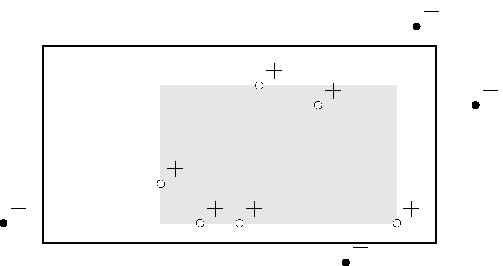
\includegraphics[scale=1]{obrazky/rectgame1.pdf}
  \caption{Obdĺžniková hra: najmenší obdĺžnik konzistentný s príkladmi.}
  \label{rectgame:hath}
\end{figure}

\begin{lemma}
  Každá množina bodov $(x_1, y_1), \ldots, (x_t, y_t)$ má unikátny
  \emph{bounding box}: najmenší (vzhľadom na inklúziu) osovorovnobežný
  obdĺžnik, ktorý ich všetky obsahuje.
\end{lemma}
\begin{proof}
  Každý obdĺžnik je jednoznačne určený $x$-ovými súradnicami ľavého
  a pravého okraja a $y$-ovými súradnicami dolného a horného okraja.
  Označme ich $x_\larr, x_\rarr$ a $y_\darr, y_\uarr$.
  Vo vnútri sú práve tie body $(x, y)$, ktoré spĺňajú
  $$x_\larr \leq x \leq x_\rarr,\ y_\darr \leq y \leq y_\uarr.$$
  Ak teda majú byť všetky spomínané body vo vnútri, musí platiť
  $$
    x_\larr \leq \min x_i,\ 
    x_\rarr \geq \max x_i,\ 
    y_\darr \leq \min y_i,\ 
    y_\uarr \geq \max y_i
  $$
  Najmenší osovorovnobežný obdĺžnik, ktorý toto spĺňa, je ten, pre
  ktorý nastávajú v jednotlivých nerovnostiach rovnosti. Teda
  $x_\larr = \min x_i$, $x_\rarr = \max x_i$, $y_\darr = \min y_i$ a $y_\uarr = \max y_i$.
\end{proof}
\begin{corollary}
  Obdĺžnik $\hat{h}$ je podmnožinou cieľového obdĺžnika $c$.
\end{corollary}
\begin{corollary}
  Obdĺžnik $\hat{h}$ je konzistentný klasifikátor.
\end{corollary}
\begin{proof}
  Konzistentnosť na pozitívnych príkladoch vyplýva z konštrukcie $\hat{h}$.
  Každý negatívny príklad je mimo $c$ a teda aj mimo $\hat{h}$, je teda
  konzistentný aj s negatívnymi príkladmi.
\end{proof}

\begin{theorem}
  Obdĺžniková hra je PAC naučiteľná: pre každý cieľový obdĺžnik $c \in C$,
  $\varepsilon > 0$, $\delta > 0$ a pravdepodobnostné rozdelenie $P$, ak
  vyššie popísanému algoritmu dáme $t$ trénovacích príkladov z $P$ a
  platí
  $$ t \geq \frac{4}{\varepsilon} \cdot \ln{\frac{4}{\delta}}, $$
  tak nám algoritmus s vysokou pravdepodobnosťou vráti hypotézu s nízkou
  chybou:
  $$ \prob(\err(\hat{h}) > \varepsilon) \leq \delta. $$
\end{theorem}
\begin{proof}
  Pod \emph{váhou} množiny budeme rozumieť pravdepodobnosť, že náhodný
  bod z rozdelenia $P$ padne do tejto množiny.
  
  Zle klasifikované body sú práve tie, ktoré sú vo vnútri $c$ ale nie sú
  vo vnútri $\hat{h}$. Každý z týchto bodov padne do aspoň jedného
  z okrajových ``pásikov'' (nerátajúc jeden z okrajov), ako je
  zobrazené na obrázku \ref{rectgame:strips}.
  Označme $p_\larr, p_\rarr, p_\uarr, p_\darr$ postupne váhy ľavého,
  pravého, horného, resp. dolného pásika, chyba $\hat{h}$ sa potom dá
  zhora odhadnúť ako súčet týchto váh:
  $$ \err(\hat{h}) \leq p_\larr + p_\rarr + p_\uarr + p_\darr. $$
  
  Ak by sme voľbou dostatočne veľkého $t$ vedeli zaručiť
  (s pravdepodobnosťou aspoň $1 - \delta$), že dostaneme takú hypotézu
  $\hat{h}$, pre ktorú je výraz na pravej strane nanajvýš $\varepsilon$,
  vyhrali by sme.
  
  Ukážeme, že vieme zaručiť (s pravdepodobnosťou aspoň $1 - \frac{\delta}{4}$)
  každú zo štyroch nerovností:
  $$ p_\larr, p_\rarr, p_\uarr, p_\darr \leq \frac{\varepsilon}{4}. $$
  Potom pravdepodobnosť, že budú všetky štyri nerovnosti platiť súčasne,
  bude aspoň $1 - \delta$, čo je presne to, čo chceme. Postup bude vo
  všetkých štyroch prípadoch ten istý, ukážeme si to teda len na ľavom pásiku.
  
  Kedy je váha ľavého pásika malá? Keď aspoň
  jeden trénovací príklad je dostatočne blízko k ľavému okraju. Keď sa
  na to pozrieme opačne, váha pásika je veľká, ak žiaden trénovací
  nie je blízko.
  Nech $\alpha$ je pravdepodobnosť toho, že trénovací príklad je blízko
  ľavého okraju. Pravdepodobnosť, že ani jeden z trénovacích príkladov
  nie je blízko, je potom $(1 - \alpha)^t \leq e^{-\alpha t}$. My chceme
  zvoliť také $t$, aby pravdepodobnosť tohto zlého prípadu bola nanajvýš
  $\frac{\delta}{4}$:
  \begin{align}
    e^{-\alpha t} &\leq \frac{\delta}{4} \\
    -\alpha t &\leq \ln{\frac{\delta}{4}} \\
    t &\geq \frac{1}{\alpha} \cdot \ln{\frac{4}{\delta}}
  \end{align}
  
  Stačí teda zvoliť $t \geq \frac{1}{\alpha} \cdot \ln{\frac{4}{\delta}}$.
  Pre úplnosť ešte ukážeme dolný odhad na pravdepodobnosť $\alpha$.
  
  Čo presne znamená byť ``dostatočne blízko'' k ľavému okraju?
  Bod $(x, y)$ je blízko, ak váha všetkých bodov naľavo od neho je
  nanajvýš $\frac{\varepsilon}{4}$. Inak zapísané,
  $$ \prob_{(x',y') \sim P} (x' < x) \leq \frac{\varepsilon}{4}.$$
  
  Vyznačme si teda všetky takéto body. Množina týchto bodov bude tvoriť
  súvislý úsek od ľavého okraja (ako na obrázku \ref{rectgame:eps_strip}),
  s tým, že hranica úseku v ňej môže ale nemusí byť. Ukážeme, že váha
  týchto bodov je aspoň $\frac{\varepsilon}{4}$, čím dostaneme odhad
  $\alpha \geq \frac{\varepsilon}{4}$. (Nie je ťažké vidieť, že ak je
  rozdelenie $P$ spojité, tak je táto váha dokonca presne
  $\frac{\varepsilon}{4}$.)
  
  \begin{figure}
    \begin{subfigure}[t]{0.49\linewidth}
      \centering
      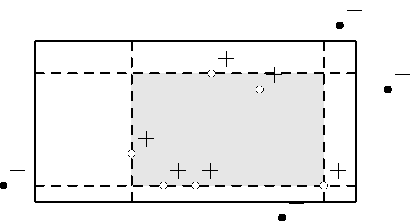
\includegraphics[scale=1]{obrazky/rectgame2.pdf}
      \caption{Krajné pásiky.}
      \label{rectgame:strips}
    \end{subfigure}
    ~
    \begin{subfigure}[t]{0.49\linewidth}
      \centering
      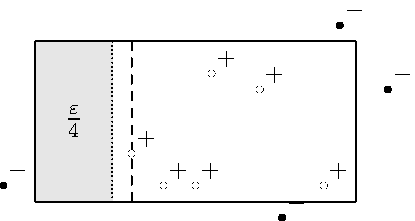
\includegraphics[scale=1]{obrazky/rectgame3.pdf}
      \caption{Sivou farbou je vyznačená množina všetkých
        bodov, pre ktoré má pásik naľavo od nich váhu nanajvýš
        $\frac{\varepsilon}{4}$.}
      \label{rectgame:eps_strip}
    \end{subfigure}
    \caption{Obdĺžniková hra.}
  \end{figure}
  
  \TODO{dôkaz (eww, grc)}
\end{proof}




\subsection{Vapnik-Chervonenkisova dimenzia}

Vapnik-Chervonenkisova dimenzia (alebo skrátene VC dimenzia) je miera
zložitosti množiny hypotéz, pomocou ktorej sme schopní tvoriť tvrdenia
v štýle PAC učenia. Na jej definíciu budeme potrebovať niekoľko pomocných
pojmov.

\begin{definition}
  Majme konečnú podmnožinu vstupov $S \subseteq X$. Hovoríme, že množina
  hypotéz $H$ \emph{rozbíja} množinu $S$, ak platí: nech označíme vstupy
  v $S$ ako pozitívne alebo negatívne akokoľvek, v množine $H$ existuje
  hypotéza konzistentná s týmto označením.
\end{definition}

Intuitívne, množina $S$ je rozbitá hypotézami $H$, ak nie je pre
hypotézy v $H$ príliš náročné modelovať príklady v $S$: sú schopné
ich modelovať akokoľvek.

\begin{definition}
  Vapnik-Chervonenkisova dimenzia množiny hypotéz $H$, označovaná
  $VCD(H)$, je veľkosť najväčšej množiny $S \subseteq X$, ktorá
  sa dá rozbiť hypotézami v $H$. Ak sa dá rozbiť ľubovoľne veľká
  množina $S$, definujeme $VCD(H) = \infty$.
\end{definition}

Teda na to, aby sme ukázali dolný odhad $VCD(H) \geq d$, stačí nám
nájsť jednu množinu $S$ veľkosti $d$, ktorá sa dá rozbiť. Aby sme ale
ukázali horný odhad $VCD(H) \leq d$, musíme ukázať, že žiadna množina
veľkosti $d + 1$ sa nedá rozbiť: teda že existuje také označenie vstupov,
pre ktoré neexistuje v $H$ konzistentný klasifikátor. Z tohto dôvodu je
obvykle ťažšie dokázať horný odhad na VC dimenziu, ako dolný odhad.

\begin{lemma}
  Majme dve množiny hypotéz $H$ a $H'$ nad tou istou množinou vstupov $x$.
  Ak platí $H \supseteq H'$, tak potom platí $VCD(H) \succeq VCD(H')$ (kde
  $\succeq$ je relácia $\geq$ prirodzene rozšírená na $\N \cup \{ \infty \}$).
\end{lemma}
\begin{proof}
  Ak sa množina $S$ dá rozbiť pomocou $H'$, potom, pretože každá hypotéza
  v $H'$ je aj v $H$, dá sa táto množina rozbiť aj pomocou $H$ (rovnakým
  spôsobom).
\end{proof}

Než uvedieme vety hovoriace o PAC naučiteľnosti, uvedieme príklady
niektorých nekonečných množín hypotéz, a neformálne zdôvodníme ich
VC dimenzie. Väčšinou budú geometrického charakteru (čo je prirodzené,
ak máme mať nekonečnú množinu hypotéz).

\paragraph{Intervaly na reálnych číslach.} Nie je ťažké vidieť, že
ľubovoľná dvojica bodov sa dá rozbiť. Na druhej strane, ak máme tri
body, tak ich vieme označiť ako na obrázku \ref{vc:interval}, čo nie
je konzistentné so žiadnym intervalom. Takže VC dimenzia je $2$.

\begin{figure}
  \centering
  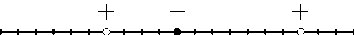
\includegraphics[scale=1]{obrazky/interval.pdf}
  \caption{Žiaden interval nevytvorí takéto označenie bodov.}
  \label{vc:interval}
\end{figure}

\paragraph{Polroviny v rovine.} Každá trojica bodov tvoriacich
nedegenerovaný trojuholník sa dá rozbiť, ako je ilustrované na
obrázku \ref{vc:halfplane}. Na druhej strane, žiadna štvorica bodov
sa rozbiť nedá: ak tvoria konvexný štvoruholník, tak jednu protiľahlú 
dvojicu označíme kladne a druhú záporne. Ak tvoria nekonvexný 
štvoruholník, jeden z bodov je vo vnútri trojuholníka tvoreného 
ostatnými tromi: tento bod označíme kladne a ostatné body záporne.
Takže VC dimenzia je $3$.

\begin{figure}
  \centering
  \begin{subfigure}[b]{0.3\linewidth}
    \centering
    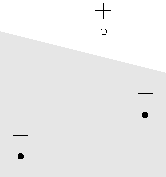
\includegraphics[scale=1]{obrazky/halfplane1.pdf}
    \caption{}
  \end{subfigure}
  ~
  \begin{subfigure}[b]{0.3\linewidth}
    \centering
    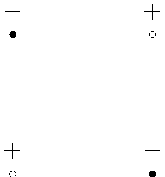
\includegraphics[scale=1]{obrazky/halfplane2.pdf}
    \caption{}
  \end{subfigure}
  ~
  \begin{subfigure}[b]{0.3\linewidth}
    \centering
    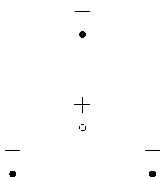
\includegraphics[scale=1]{obrazky/halfplane3.pdf}
    \caption{}
  \end{subfigure}
  \caption{Polroviny v rovine: v situácii (a) vieme nájsť deliacu priamku, v (b) a (c) nie.}
  \label{vc:halfplane}
\end{figure}

\paragraph{Osovorovnobežné obdĺžniky.} Štvorica bodov, ktorá sa dá
rozbiť, je ilustrovaná na obrázku \ref{vc:rect}, nie každá štvorica
bodov sa ale dá rozbiť. Na druhej strane, žiadna pätica bodov sa nedá
rozbiť. Rozoberieme dva prípady: ak je aspoň jeden z bodov vo vnútri 
bounding boxu (nie na okraji), tak ho označíme záporne a všetky body na 
okraji kladne. Ak sú všetky body na obvode bounding boxu, na jednej 
strane toho obdĺžnika musia ležať aspoň dva body. Jeden z nich označíme 
kladne a druhý záporne. Takže VC dimenzia je $4$.

\begin{figure}
  \centering
  \begin{subfigure}[b]{0.23\linewidth}
    \centering
    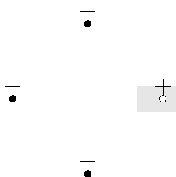
\includegraphics[scale=1]{obrazky/vc_rect1.pdf}
    \caption{}
  \end{subfigure}
  ~
  \centering
  \begin{subfigure}[b]{0.23\linewidth}
    \centering
    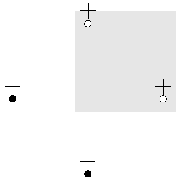
\includegraphics[scale=1]{obrazky/vc_rect2.pdf}
    \caption{}
  \end{subfigure}
  ~
  \centering
  \begin{subfigure}[b]{0.23\linewidth}
    \centering
    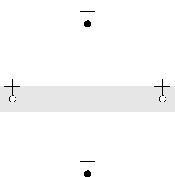
\includegraphics[scale=1]{obrazky/vc_rect3.pdf}
    \caption{}
  \end{subfigure}
  ~
  \centering
  \begin{subfigure}[b]{0.23\linewidth}
    \centering
    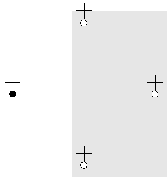
\includegraphics[scale=1]{obrazky/vc_rect4.pdf}
    \caption{}
  \end{subfigure}
  \caption{Osovorovnobežné obdĺžniky: štvorica bodov, ktorá sa dá rozbiť.
    Jednotlivé obrázky zobrazujú všetky netriviálne označenia bodov a
    príslušné konzistentné klasifikátory.}
  \label{vc:rect}
\end{figure}

\medskip

Nakoniec hlavný výsledok, kvôli ktorému je VC dimenzia zaujímavá.

\begin{theorem}[Blumer et. al., 1989 \cite{blumer1989learnability}]
  Nech $C$ je ľubovoľná množina konceptov. Nech $H$ je množina hypotéz
  s VC dimenziou rovnou $d$. Nech $L$ je ľubovoľný algoritmus, ktorý
  pre ľubovoľnú sadu $t$ trénovacích príkladov vráti hypotézu $\hat{h}$
  konzistentnú s príkladmi. Potom $L$ je PAC trénovací algoritmus pre
  množinu konceptov $C$ s použitím hypotéz v $H$, pokiaľ je $t$
  dostatočne veľké:
  $$ t \geq c_0 \left( \frac{1}{\varepsilon} \ln{\frac{1}{\delta}} + \frac{d}{\varepsilon} \ln{\frac{1}{\varepsilon}} \right) $$
  pre nejakú konštantu $c_0 > 0$.
\end{theorem}

\TODO{dôkaz}

\begin{theorem}[Haussler et. al., 1994 \cite{haussler1994predicting}]
  Ak VC dimenzia je $d$, tak ľubovoľný trénovací algoritmus, ktorý vždy
  vracia hypotézy konzistentné s trénovacími príkladmi, má chybu nanajvýš
  $$ \E \left[ \err(\hat{h}) \right] = O\left( \frac{d}{t} \ln{\frac{t}{d}} \right). $$
\end{theorem}

\TODO{dôkaz}

Čo ale v prípade, že neexistuje konzistentný klasifikátor? Taká situácia
nastane, keď buď cieľový koncept nie je v množine hypotéz, alebo keď v
probléme vystupuje šum. Ukazuje sa, že aj v takom prípade sa dá
odhadnúť chyba hypotézy.

\begin{theorem}[Vapnik \& Chervonenkis, 1971 \cite{chervonenkis1971theory}]
  Nech $h^\star$ je hypotéza v $H$ s najmenšou (testovacou) chybou a
  nech $\hat{h}$ je hypotéza v $H$ s najmenšou trénovacou chybou. Ak
  $VCD(H) = d$, tak pre počet trénovacích príkladov
  $$ t \geq c_0 \left( \frac{1}{\varepsilon} \ln{\frac{1}{\delta}} + \frac{d}{\varepsilon} \ln{\frac{1}{\varepsilon}} \right), $$
  kde $c_0$ je nejaká konštanta, platí, že s veľkou pravdepodobnosťou
  je chyba hypotézy $\hat{h}$ dostatočne malá (berúc v úvahu najmenšiu
  dosiahnuteľnú chybu):
  $$ \prob( \err(\hat{h}) > \err(h^\star) + \varepsilon ) \leq \delta. $$
\end{theorem}

\TODO{dôkaz}

  
  \bibliographystyle{plain}
  \bibliography{literatura} 
  
\end{document}
